\documentclass[aps,physrev,reprint,superscriptaddress,nofootinbib,twocolumn]{revtex4-2}
\usepackage{amsmath}
\usepackage{graphicx}
\usepackage[caption=false]{subfig}
  \captionsetup[subfigure]{position=top,
                           textfont=normalfont,
                           singlelinecheck=off,
                           justification=raggedright
                           }
\usepackage{fontawesome}
\usepackage{tikz}
  \usetikzlibrary{arrows.meta,calc,shapes}
\usepackage{pifont}
  \newcommand{\vmark}{\text{\ding{51}}}
  \newcommand{\xmark}{\text{\ding{55}}}
\usepackage[hidelinks]{hyperref}

\begin{document}
\title{Symmetric observations without symmetric causal explanations}
\author{Christian William}
\affiliation{Department of Applied Physics, University of Geneva, 1211 Geneva 4, Switzerland}
\author{Patrick Remy}
\affiliation{Department of Applied Physics, University of Geneva, 1211 Geneva 4, Switzerland}
\author{Jean-Daniel Bancal}
\affiliation{Universit\'e Paris-Saclay, CEA, CNRS, Institut de physique th\'eorique, 91191, Gif-sur-Yvette, France}
\author{Yu Cai}
\affiliation{School of Physical and Mathematical Sciences, Nanyang Technological University, Singapore 637371}
\author{Nicolas Brunner}
\affiliation{Department of Applied Physics, University of Geneva, 1211 Geneva 4, Switzerland}
\author{Alejandro Pozas-Kerstjens}
\thanks{physics\faAt{}alexpozas.com}
\affiliation{Department of Applied Physics, University of Geneva, 1211 Geneva 4, Switzerland}

\begin{abstract}
    Inferring causal models from observed correlations is a challenging task, crucial to many areas of science.
    In order to alleviate the effort, it is important to know whether symmetries in the observations correspond to symmetries in the underlying realization.
    Via an explicit example, we answer this question in the negative.
    We use a tripartite probability distribution over binary events that is realized by using three (different) independent sources of classical randomness.
    We prove that even removing the condition that the sources distribute systems described by classical physics, the requirements that i) the sources distribute the same physical systems, ii) these physical systems respect relativistic causality, and iii) the correlations are the observed ones, are incompatible.
\end{abstract}

\maketitle

In understanding all, the response of electric current with temperature in a material, the behavior of a flock against a predator, or the effect of a social policy in well-being, capturing which events cause which others and what are the causation mechanisms are arguably the most fundamental questions that one can ask.
Despite its primary importance as a core component of the scientific process, an operational approach to causal inference has only been developed reasonably recently \cite{causalitybook,spirtesbook}.

Modern approaches to causal inference, aided by improvements in computational capability, resort to discrete search techniques over the space of possible causal mechanisms.
A standard procedure is constraint-based: beginning with fully connected causal graphs, the independence relations extracted from the data are used to prune connections \cite{pasquato2023}.
Alternatively, there also exist score-based techniques, that rank each causal explanation by the likelihood that it can generate the observations \cite{jin2024}.
In both approaches, a strong desideratum is to restrict the search space as much as possible.

Therefore, the question of understanding the level of symmetry in observations compared to the level of symmetry in the underlying model becomes central.
Yet, it is challenging to answer it, since observations and their realizations are very different objects.
Indeed, while it is intuitively clear (see Fig.~\ref{fig:setting} and the discussions below) that symmetries in a causal process lead to corresponding symmetries at the level of observable events, for some given observations with some symmetries there might be several causal explanations, and not all of them (if any) might have corresponding symmetries.

\begin{figure}
    \centering
    \subfloat[\label{fig:triangleDAG}]{
        \scalebox{0.7}{
          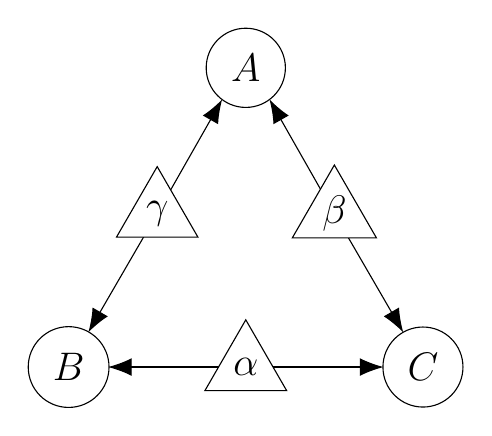
\begin{tikzpicture}
            \draw [-{Latex[length=3mm]}] (2.6, 0) -- (4., 0);
            \draw [{Latex[length=3mm]}-] (0.5, 0) -- (2.1, 0);
            \draw [-{Latex[length=3mm]}] (1.125, 1.949) -- (0.25, 0.44);
            \draw [-{Latex[length=3mm]}] (1.125, 1.949) -- (1.95, 3.4);
            \draw [{Latex[length=3mm]}-] (2.55, 3.4) -- (3.375, 1.949);
            \draw [-{Latex[length=3mm]}] (3.375, 1.949) -- (4.25, 0.44);
            \node[draw,fill=white,circle,inner sep=5pt] at (2.25, 3.8) {\Large$A$};
            \node[draw,fill=white,circle,inner sep=5pt] at (0, 0) {\Large$B$};
            \node[draw,fill=white,circle,inner sep=5pt] at (4.5, 0) {\Large$C$};
            \node[draw,fill=white,regular polygon, regular polygon sides=3,inner sep=1.5pt] at (2.25, 0) {\Large$\alpha$};
            \node[draw,fill=white,regular polygon, regular polygon sides=3,inner sep=1.5pt] at (1.125, 1.949) {\Large$\gamma$};
            \node[draw,fill=white,regular polygon, regular polygon sides=3,inner sep=-0.2pt] at (3.375, 1.949) {\Large$\beta$};
          \end{tikzpicture}
      }
    }
    \hspace{0.5cm}
    \subfloat[\label{fig:setting}]{
        \scalebox{0.7}{
          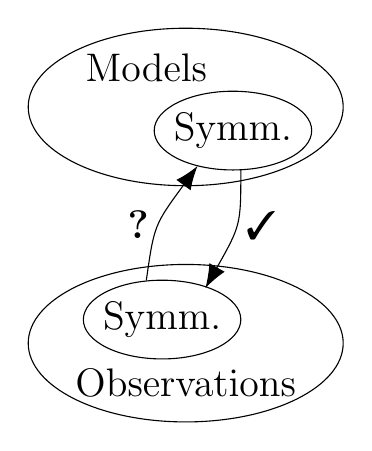
\begin{tikzpicture}
            % Top ovals
            \draw[fill=white] (0,2) ellipse (2cm and 1cm);
            \node at (-0.5,2.5) {\Large Models};
            \draw[fill=white] (0.6,1.7) ellipse (1cm and 0.5cm) node {\Large Symm.};
            
            % Bottom ovals
            \draw[fill=white] (0,-1) ellipse (2cm and 1cm);
            \node at (0,-1.5) {\Large Observations};
            \draw[fill=white] (-0.3,-0.7) ellipse (1cm and 0.5cm) node {\Large Symm.};
            
            % Curved arrows
            \draw[-{Latex[length=3mm]},>=stealth] (0.7,1.2) .. controls (0.7,0.5) .. (0.25,-0.3) node[midway,right] {\Large\vmark};
            \draw[-{Latex[length=3mm]},>=stealth] (-0.5,-0.2) .. controls (-0.4,0.5) .. (0.15,1.25) node[midway,left] {\Large\textbf{?}};
          \end{tikzpicture}
        }
    }
    \caption{
        \protect\subref{fig:triangleDAG} The triangle causal structure.
        Three bipartite latent variables, $\alpha$, $\beta$ and $\gamma$ influence each a different set of two out of the three visible variables $A$, $B$ and $C$.
        This structure has received considerable attention in the context of nonlocality in quantum networks.
        \protect\subref{fig:setting} Pictorial representation of the relations between realizations and observations.
        In this work we demonstrate that $\textbf{?}=\xmark$.
        Namely, there exist probability distributions over the binary-valued observations that i) are produced in the triangle causal structure by classical physical systems and ii) are invariant under permutations of the visible nodes, yet they do not admit explanations in terms of symmetric models, i.e., when $\alpha$, $\beta$ and $\gamma$ denote copies of a same physical system. 
        }
    \label{fig:intro}
\end{figure}

In this work we demonstrate that symmetries in observations cannot be always translated into corresponding symmetries in the causal mechanism that produces such observations.
Since it is known that different physical theories allow to produce different types of observations under the same causal mechanism \cite{bell1964}, we take a conservative approach and only demand consistency with relativistic causality.
Thus, our results are a proof that there exist observations that, despite presenting some observable symmetries, cannot be created by causal mechanisms that satisfy the corresponding symmetries in any physical theory consistent with relativistic causality.

\paragraph*{Observations vs. realizations.---}
Our aim is to shed light on the relation between symmetries in observations and symmetries in the underlying causal model.
For doing so, we focus on a simple scenario with three binary observed variables, where each pair is influenced by an independent latent variable (see Fig.~\ref{fig:triangleDAG}).
This is known as the triangle scenario, and has received considerable attention in the context of Bell nonlocality \cite{TavakoliPozas2022,fritz2012,renou2019,fraser2018,gisin2020,pozas2023}.

In the context of Bayesian probability theory, all nodes in Fig.~\ref{fig:triangleDAG} represent random variables, and the arrows indicate a functional dependence.
Under the lens of quantum information theory, this is precisely the physical realization of network local models \cite{fritz2012,TavakoliPozas2022}, i.e., this interpretation of the nodes and arrows leads to the characterization of the observations that are generated by measuring physical systems whose dynamics are described by classical mechanics \cite{wood2015}.
This opened the door to an extended interpretation of the graphs such as that in Fig.~\ref{fig:triangleDAG}, where the latent nodes describe physical systems that are distributed to parties, represented by the visible nodes \cite{Henson2014,Weilenmann2020}.
On the received physical systems, each party performs a measurement in order to produce the concrete value of their variable in a given round.

The concrete expression for the calculation of the probabilities of the different events, thus, has a dependence on the physical theory assumed to govern the systems distributed.
For classical systems, the expression for calculating probabilities of observable events is given by the Markov condition\footnote{The Markov condition states that the value of any variable in the graph depends only by the value of the variables that have a direct influence on it.}.
In the case of the systems being described by quantum mechanics, it is Born's rule.
These are nothing but particular cases of what has evolved into an information-theoretic perspective of physics, known as generalized probabilistic theories (GPT) \cite{janotta2014,plavala2023,Weilenmann2020}.
In this theory-agnostic formulation, observations created by the causal mechanism in Fig.~\ref{fig:triangleDAG} are described by
\begin{equation}
    \begin{aligned}
        p(A&=a,B=b,C=c) \\
        &= e^a_{A_1A_2}\otimes f^b_{B_1B_2}\otimes g^c_{C_1C_2}\left(\alpha_{B_2C_1}\otimes\beta_{C_2A_1}\otimes\gamma_{A_2B_1}\right),
    \end{aligned}
    \label{eq:GPT}
\end{equation}
where the subscripts denote vector spaces, $\alpha$, $\beta$ and $\gamma$ (the \textit{states} distributed by the latent nodes) are elements of a tensor product of the corresponding spaces, and $e^a$, $f^g$ and $g^c$ (the \textit{effects} that describe the measurements performed by the parties) are elements of the dual of the tensor product of the corresponding spaces, all satisfying suitable properties \cite{ludwigbook,krausbook}.
From now on, we will use the shorthand notation $p(a,b,c)=p(A=a,B=b,C=c)$.

Consider now the symmetric version of the scenario, where the three latent nodes now distribute copies of the same state, $\omega$, and all the parties perform the same effect, $e$ (see Fig.~\ref{fig:triangle}).
The model for distributions observed in this situation has the form
\begin{equation}
    p(a,b,c)\!=\!e^a_{A_1A_2}\otimes e^b_{B_1B_2}\otimes e^c_{C_1C_2} \!\left(\omega_{A_2B_1}\!\otimes\omega_{B_2C_1}\!\otimes\omega_{C_2A_1}\right)\!.
    \label{eq:symmGPT}
\end{equation}
Importantly, in this equation, permuting the labels $A$, $B$ and $C$ leads to the exact same expression.

Now consider the parameterization of the distributions above.
If the visible variables are binary, $a,\,b,\,c\in\{-1,1\}$, an arbitrary probability distribution $p(a,b,c)$ is characterized by seven independent parameters\footnote{Namely all probabilities minus the normalization constraint.}.
However, for distributions that are generated via Eq.~\eqref{eq:symmGPT}, the symmetry reduces this number to just three parameters: every tripartite distribution over binary variables that is symmetric under permutation of the parties can be expressed as
\begin{equation}
    \begin{aligned}
        p(a,b,c)=\,&\frac18\left[ 1+(a+b+c)E_1\right.\\
        &\quad\,\,\,\left.\,+(ab+ac+bc)E_2+abcE_3\right],
        \end{aligned}
    \label{eq:prob}
\end{equation}
for some $E_1$, $E_2$, $E_3\in[-1,1]$.
In short, the causal model given by Eq.~\eqref{eq:symmGPT} implies that the observed distribution can be expressed via Eq.~\eqref{eq:prob}.
This is pictorially captured in the downward-pointing arrow in Fig.~\ref{fig:setting}.

Here we ask the opposite question: if we have a realization (in the sense of Eq.~\eqref{eq:GPT}) that produces a distribution invariant under permutation of parties (i.e., of the form of Eq.~\eqref{eq:prob}), can we always find an alternative symmetric realization of the form of Eq.~\eqref{eq:symmGPT}?

Previous works have touched upon this question in the context of classical realizations \cite{gisin2020,silva2023}.
Surprisingly, answers point towards opposite conclusions: on the one hand, the classical model (given in the Supplementary Note 2 of \cite{gisin2020}) for the probabilistic mixture of a uniform shared random bit with the least amount of white noise that makes the distribution known to be producible in the triangle scenario with classical sources is symmetric.
On the other hand, the analogous study for the distribution where uniformly all but one of the parties produce a given output (known as the W distribution) showed that in this case the model was asymmetric \cite{silva2023}, reporting not being able to achieve the same results even with larger symmetric models.

Our work settles this apparent discrepancy by proving a strong version of the latter observation.
Namely, we give a family of tripartite probability distributions over binary variables that i) can be produced in the triangle scenario when the sources distribute systems described by classical physics and ii) are invariant under permutations of parties, that we prove are impossible to reproduce with symmetric strategies and any physical systems that are consistent with relativity.
This includes theoretical, stronger-than-quantum systems \cite{Henson2014,janotta2014,plavala2023}.

\paragraph*{The distribution.---}
The example that we use comes from the study of quantum nonlocality in networks \cite{TavakoliPozas2022} in the triangle scenario. 
It is the family of distributions of the form given in Eq.~\eqref{eq:prob} with $E_1=E_1^c\approx0.1753$ (the exact form of $E_1^c$ is given in Appendix \ref{app:E_1c}) and $E_2=-1/3$.
For these values of $E_1$ and $E_2$, positivity of Eq.~\eqref{eq:prob} for any $a,b,c$ fixes $E_3=E_3^c\approx-0.5260$.
However, our proof technique does not use this information, so when we consider different values of $E_1$ and $E_2$ later on, the proofs will hold for any value of $E_3$ that leads to a well-defined probability distribution.
Appendix~\ref{app:model} contains a triangle-local model for this distribution (see also Ref.~\cite{gisin2020}).

\paragraph*{Proof for $E_1\,{=}\,E_1^c$, $E_2\,{=}\,{-}1/3$.---} 
We will prove the impossibility of generating any distribution \eqref{eq:prob} for $E_1=E_1^c$ and $E_2=-1/3$ with symmetric realizations in the triangle scenario via reduction to the absurd.
Thus, let us initially assume that the distribution admits a realization, i.e., that there exists a source of bipartite physical systems $\omega$, and a measurement device characterized by the effect $e$ that produces a classical bit out of processing two input systems, which, when three copies of each are arranged in the triangle-like structure of Fig.~\ref{fig:triangle}, the possible outcomes are produced according to Eq.~\eqref{eq:prob} with $E_1=E_1^c$ and $E_2=-1/3$.
If that were indeed the case, one could take not just three but, say, seven copies of the source and the measurement device, and arrange them forming a heptagon, as in Fig.~\ref{fig:inflation}.
In this scenario, the measurements produce outcomes $a_0,\dots,a_6\in\{-1,1\}^7$ according to a distribution $p_\text{inf}(a_0,\dots,a_6)$.

\begin{figure}
    \centering
    \subfloat[\label{fig:triangle}]{
        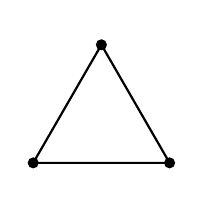
\begin{tikzpicture}
            \node[] at (0,0) {};
            \draw[thick,rotate=90,xshift=-1.1cm] (0:1) \foreach \x in {120,240} { -- (\x:1) } -- cycle;
            \foreach \x in {0,120,240} {
                \fill[black,rotate=90,xshift=-1.1cm] (\x:1) circle (2pt);
            }
        \end{tikzpicture}
    }
    \hspace{2cm}
    \subfloat[\label{fig:inflation}]{
        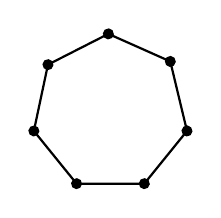
\begin{tikzpicture}
            \draw[thick,rotate=40.5] (0:1) \foreach \x in {51,102,...,309} { -- (\x:1) } -- cycle;
            \foreach \x in {0,51,102,...,309} {
                \fill[black,rotate=40.5] (\x:1) circle (2pt);
            }
        \end{tikzpicture}
    }
    \caption{
        \protect\subref{fig:triangle} simplified representation of the triangle DAG in Fig.~\ref{fig:triangleDAG} for symmetric causal scenarios.
        Each line represents an independent copy of a same bipartite state $\omega$, that is distributed to the two parties (the nodes) that it is connected to.
        All parties perform the same measurement, given by the effect $\{e^o\}_o$, to produce their outcomes.
        Any process following this causal mechanism leads to distributions over the observable events that are invariant under permutations of the observable nodes.
        For all observations that are produced in this way, one can consider the distributions that are created when using more copies of the state and the measurement device like, for instance, that in \protect\subref{fig:inflation}.
        We use the consistency conditions implied by the existence of this distribution to prove that the distribution with $E_1=E_1^c$, $E_2=-1/3$, and $E_3=E_3^c$ is impossible to generate in the symmetric triangle network under any physical theory consistent with relativity.
        }
\end{figure}

This distribution has several properties.
First, since it is a probability distribution, all the probabilities must be non-negative and sum to 1.
Second, since all the sources and measurement devices are the same, it is invariant under any cyclic permutation of the parties, i.e.,
\begin{equation}
    p_\text{inf}(a_0,\dots,a_6)=p_\text{inf}(a_{i},\dots,a_{6\oplus i})\quad\forall i=1,\dots,6,
    \label{eq:symm}
\end{equation}
where the $\oplus$ symbol represents addition modulo 7.
Third, since the sources and measurement devices used in creating $p_\text{inf}$ are the same as those used for creating $p$, the two-body marginals (and hence the one-body marginals) of both distributions must be the same.
This, in particular, implies that
\begin{equation}
    \begin{aligned}
        \sum_{a_0,a_2}p_\text{inf}&(a_0,a_1,a_2,a_3,a_4,a_5,a_6)\\
        =\frac{1}{2}&\left(1+a_1 E_1^c\right)\sum_{a'_0,a'_1,a'_2}p_\text{inf}(a'_0,a'_1,a_2',a_3,a_4,a_5,a_6)\\
        &\hspace{4.5cm}\forall a_1,a_3,a_4,a_5,a_6,\\
        \sum_{a_0,a_3}p_\text{inf}&(a_0,a_1,a_2,a_3,a_4,a_5,a_6)\\
        =&\frac{1}{4}\left[1+\left(a_1+a_2\right)E_1^c-\frac{1}{3}a_1 a_2\right]\\
        &\times\!\!\!\!\sum_{a'_0,a'_1,a'_2,a'_3}\!\!\!\!p_\text{inf}(a'_0,a_1',a_2',a_3',a_4,a_5,a_6)\\
        &\hspace{4.5cm}\forall a_1,a_2,a_4,a_5,a_6.
    \end{aligned}
    \label{eq:iden}
\end{equation}

Equations~\eqref{eq:symm} and \eqref{eq:iden} are linear in the probabilities $p_\text{inf}(a_0,\dots,a_6)$.
This means that determining the existence of a $p_\text{inf}(a_0,\dots,a_6)$ that satisfies the necessary properties is an instance of a linear program \cite{boydbook}.
In the computational appendix \cite{compapp} we set up this linear program and show that it is infeasible, i.e., that a collection of non-negative numbers $\{p_\text{inf}(a_0,\dots,a_6)\}_{a_0,\dots,a_6\in\{-1,1\}}$ that, simultaneously, sum to one and satisfy Eqs.~\eqref{eq:symm} and \eqref{eq:iden} does not exist.
Recall that such a collection should exist if the original distribution $p(a,b,c)$ given in Eq.~\eqref{eq:prob} was possible to create with a symmetric strategy in the triangle scenario.
Thus, we have a proof that none of the probability distributions given by Eq.~\eqref{eq:prob} for $E_1=E_1^c$ and $E_2=-1/3$ admits a symmetric realization.

At this point, two facts must be highlighted: i) it is known that the distribution \eqref{eq:prob} with $E_1=E_1^c$, $E_2=-1/3$ and $E_3\approx-0.5260$ can be realized with a non-symmetric strategy when the sources distribute physical systems obeying the rules of classical physics, and ii) we have not requested any special property to the sources in our symmetric construction.
In particular, we have not demanded that they distribute physical systems described according to any particular physical theory.
Thus, our result is a proof that symmetries in a probability distribution not always translates to symmetries in its realization: while Eq.~\eqref{eq:prob} with $E_1=E_1^c$, $E_2=-1/3$ and $E_3\approx-0.5260$ is symmetric under permutations of parties and can be realized in the triangle scenario classically, neither by using physical systems described by classical, quantum, or potentially stronger-than-quantum physics, it will be possible to realize in setups where all sources and measurement devices are equal.

\paragraph*{Systematic approach.---}
The proof above is an instance of the inflation argument.
Inflation has turned out to be a powerful tool for characterizing the probability distributions that can be produced in causal scenarios with latent nodes that distribute classical \cite{wolfe2019,pozas2022b,pozas2023,fraser2018,lauand2024,lauand2023}, quantum \cite{wolfe2021,pozas2023}, and arbitrary physical systems \cite{gisin2020,camillo2023}, as well as scenarios with different sources being of different types \cite{pozas2022,wang2023}.
Its success is, in part, due to its applicability to any causal structure, and in part due to the fact that it relaxes the sets of correlations under study to forms amenable to linear or semidefinite programming \cite{TavakoliPozas2024}, that can be solved in many cases with standard computational resources \cite{boghiu2022,TavakoliPozas2024}.
Moreover, it is possible to define hierarchies of inflation relaxations \cite{navascues2017,wolfe2021,ligthart2023}, that in some cases are known to converge \cite{navascues2017,ligthart2023,ligthart2023b}.

\begin{figure}
    \centering
    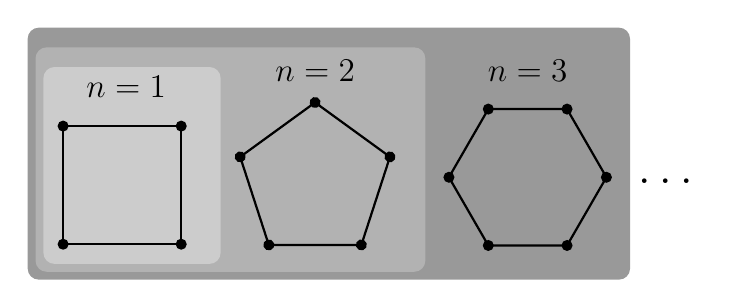
\begin{tikzpicture}
    
    % Colors
    \definecolor{lightgray}{gray}{0.8}
    \definecolor{mediumgray}{gray}{0.7}
    \definecolor{darkgray}{gray}{0.6}
    
    % Rectangles
    \fill[darkgray,rounded corners] (-0.45,-0.45) rectangle (7.2,2.75);
    \fill[mediumgray,rounded corners] (-0.35,-0.35) rectangle (4.6,2.5);
    \fill[lightgray,rounded corners] (-0.25,-0.25) rectangle (2,2.25);
    \draw[thick] (0,0) -- (1.5,0) -- (1.5,1.5) -- (0,1.5) -- cycle;

    % Square
    \foreach \x in {0,1.5} {
        \foreach \y in {0,1.5} {
            \fill[black] (\x,\y) circle (2pt);
        }
    }
    
    % Pentagon
    \draw[thick,xshift=3.2cm,yshift=0.8cm,rotate=18] (0:1) \foreach \x in {72,144,...,288} { -- (\x:1) } -- cycle;
    \foreach \x in {0,72,...,288} {
        \fill[black,xshift=3.2cm,yshift=0.8cm,rotate=18] (\x:1) circle (2pt);
    }
    
    % Hexagon
    \draw[thick,xshift=5.9cm,yshift=0.85cm] (0:1) \foreach \x in {60,120,...,300} { -- (\x:1) } -- cycle;
    \foreach \x in {0,60,...,300} {
        \fill[black,xshift=5.9cm,yshift=0.85cm] (\x:1) circle (2pt);
    }

    % Labels
    \node[] at (7.7,0.8) {\LARGE$\dots$};
    \node[] at (0.8,2) {\large$n=1$};
    \node[] at (3.2,2.2) {\large$n=2$};
    \node[] at (5.9,2.2) {\large$n=3$};
    
    \end{tikzpicture}
    \caption{
        Depiction of the hierarchy of inflations that we use.
        In each level, we demand the existence of probability distributions for each of the networks with smaller number of nodes too.
        These distributions are related to each other by constraints on the marginals over a same number of nodes (see Eq.~\eqref{eq:iden}).}
    \label{fig:hierarchy}
\end{figure}

In our case of interest, it is possible to define an inflation hierarchy of compatibility conditions with symmetric realizations, which we pictorially illustrate in Fig.~\ref{fig:hierarchy}.
Step $n$ in the hierarchy demands the existence of $n$ probability distributions, $\{p_k(a_0,\dots,a_k)\}_{k=4}^{n+3}$, all of them symmetric under cyclic permutations (i.e., satisfying the analogues of Eq.~\eqref{eq:symm}), and each of them compatible (in the sense of Eq.~\eqref{eq:iden}) with the distribution under test \cite{girardin2023}.
Since all the sources and measurement devices in all inflations are required to be identical, the distributions are related to each other via
\begin{equation}
    \sum_{a_{k-1},a_k}p_k(a_0,\dots,a_k) = \sum_{a_{k-1}}p_{k-1}(a_0,\dots,a_{k-1})
\end{equation}
for all $a_0,\dots,a_{k-2}$.

Using a standard tabletop computer ($\sim1$ GB of RAM) it is possible to run up to the 11th level of the hierarchy (i.e., up to the inflation with 14 nodes) in a few seconds per distribution, producing the orange area in Fig.~\ref{fig:results}, that denotes symmetric distributions that do not admit symmetric realizations.
Using $\sim50$ GB of RAM and around 1 day of computation time, we are able to certify that all distributions of the form of Eq.~\eqref{eq:prob} for $E_2=-1/3$ are impossible to realize with arbitrary symmetric strategies for $E_1\geq0.1580$ and any allowed value of $E_3$ (the red circle in Fig.~\ref{fig:results}), using the 15th level of the hierarchy.

\paragraph*{Certificates of incompatibility.---}
A convenient property of linear programs is Farkas' lemma, which states that every linear program either has a solution or there exists a certificate (findable by linear programming) that there is no solution.
In the context of inflation, certificates of infeasibility can generally be understood as Bell-like inequalities \cite{bell1964} that separate (relaxations of) the set of distributions that can be produced in a given scenario from (a subset of) those that cannot.

The constraints \eqref{eq:iden} are known in the literature as linearized polynomial constraints \cite{pozas2022b,alexthesis}, and they are examples of constraints that lead to certificates of infeasibility that are only applicable to the distribution under scrutiny \cite{pozas2022b}.
In order to obtain certificates that apply to other distributions, one can either follow the prescriptions of \cite{pozas2022b}, or can alternatively relax Eq.~\eqref{eq:iden} to constraints on only the marginals that can be associated to (products of) marginals in the original network.
For instance, in the inflation in Fig.~\ref{fig:inflation}, these constraints are
\begin{equation}
    \begin{aligned}
        \sum_{a_2,a_5,a_6}\!\! p_\text{inf}(a_0,\dots,a_6)=\frac{1}{16} &\left[1+(a_0+a_1)E_1+a_0a_1E_2\right]\\
        \times&\left[1+(a_3+a_4)E_1+a_3a_4E_2\right],\\
        \sum_{a_2,a_4,a_6}\!\! p_\text{inf}(a_0,\dots,a_6) =\frac{1}{16} &\left[1+(a_0+a_1)E_1+a_0a_1E_2\right]\\
        \times&\left(1+a_3E_1\right)\left(1+a_5E_1\right).
    \end{aligned}
    \label{eq:nolpi}
\end{equation}
Replacing the constraints \eqref{eq:iden} with \eqref{eq:nolpi} and running the respective linear programs, we are able to determine the infeasibility of distributions for $E_2=-1/3$ only for $E_1\geq0.1656$ using the 15th level of the hierarchy.
In exchange, we obtain a witness of incompatibility with symmetric realizations in the triangle, which is the upper boundary to the dark green region in Fig.~\ref{fig:results}.
The expression of this certificate is given in Appendix \ref{app:cert}, and stored in machine-readable form in the computational appendix \cite{compapp}.

\begin{figure}
    \centering
    \includegraphics[width=0.95\linewidth]{results.pdf}
    \caption{Projection of the space of probability distributions given by Eq.~\eqref{eq:prob} on the plane defined by $E_1$ and $E_2$.
    The points in the gray area produce negative probabilities for any value of $E_3$.
    The points in the blue area correspond to distributions that cannot be generated in the triangle scenario, regardless of the nature of the sources \cite{gisin2020}.
    In the area to the left of the yellow boundary for every $E_1$ and $E_2$ there exists at least one value of $E_3$ for which the corresponding distribution admits a realization in the triangle structure with classical latent variables \cite{gisin2020}.
    In particular, the blue triangle denotes the distribution that we use in the work, with $E_1=E_1^c\approx0.1753$ and $E_2=-1/3$.
    The orange area denotes the distributions that are proven not to admit a symmetric realization in the triangle scenario using the 11th level of the corresponding inflation hierarchy using the constraints of the type of Eq.~\eqref{eq:iden}.
    Using $\sim50$ GB of RAM and one day of compute we are able to identify as incompatible also the point denoted with a red circle ($E_1=0.1580$ and $E_2=-1/3$) using the 15th level of the hierarchy.
    The dark green area contains the distributions that are identified as incompatible by the certificate obtained by substituting the constraints \eqref{eq:iden} by \eqref{eq:nolpi} and testing the distribution with $E_1=0.1656$ and $E_2=-1/3$.
    The expression of the certificate is given in Appendix \ref{app:cert}.
    }
    \label{fig:results}
\end{figure}

\paragraph*{Discussion.---}
In physics, symmetries allow to gain a better understanding of the concrete process under study.
However, there exist cases where the symmetries appear to be emergent, in the sense that the macroscopic observations have a symmetry that is not present in the currently available microscopic model of the phenomenon.
An example of this can be found in the context of hydrodynamic turbulence, where some phenomena appear to have scale invariance despite the underlying Navier-Stokes equations not possessing such symmetry \cite{frisch1995turbulence,shavit2022}.

The results in this work demonstrate a strong version of these observations: there exist distributions over measurable events that have a macroscopic symmetry (in our case, under permutations of the measured variables), for which we prove that a realization in terms of a symmetric causal model is impossible in any physical theory.
In other words, the conditions of symmetry in observable events, symmetry in the causal mechanism that produces such events, and relativistic causality, are not always all compatible.

From a pure causal inference perspective, when looking for causal explanations of observations, it is desirable to reduce the search space as much as possible.
Our results indicate that symmetries in the observed data cannot be used for this purpose.
On a more positive side, we have built a hierarchy of simple tests that may be useful for certification purposes.
The reason for this is that the failure of any of them constitutes a proof that the observed statistics cannot be produced in the model under scrutiny.
This may have applications in cryptography, where the parties may want to guarantee some properties of the setup while potentially not trusting each other.

While illustrated in this work for the triangle causal structure, an analogous approach can be followed for more complex scenarios.
One could also follow the same procedure to impose symmetries only in specific parts of the model, in analogy with the approach that is followed to characterize the distributions generated in scenarios where the different sources distribute systems described by different physical theories \cite{wolfe2021,pozas2022}.
Following this line of research, it would be interesting to characterize more fine-grained symmetries, such as measurement devices that do not distinguish between input ports.

\acknowledgments
We thank Fernando Parisio and Bastien Chopard for helpful discussions and comments.
This work is supported by the National Research Foundation, Singapore under its Quantum Engineering Programme (National Quantum-Safe Network, NRF2021-QEP2-04-P01) and the Swiss National Science Foundation (grant numbers 192244 and 224561).
Computations were performed in part at the University of Geneva using the Baobab HPC service.

\appendix
\onecolumngrid
\section{The example distribution}
\label{app:E_1c}
The distribution that we use throughout the work is initially described in the Supplemental Materials of Ref.~\cite{gisin2020}.
It corresponds to the distribution with $E_2=-1/3$ that has the highest value of $E_1$ while being producible when the latent nodes represent sources of physical systems described by classical mechanics.
This value, which we call $E_1^c$ in the main text, is
\begin{equation*}
    \begin{aligned}
        E_1^c=&\,\frac{1}{2} 
        -\frac{1}{6\sqrt{\frac{3}{3\ 2^{5/3}\sqrt[3]{3\sqrt{41} + 25} + \sqrt[3]{21600 - 2592\sqrt{41}} - 21}}} \\
        &+ \frac{1}{2}\sqrt{\frac{34}{\sqrt{3\left(3\ 2^{5/3}\sqrt[3]{3\sqrt{41} + 25} + \sqrt[3]{21600 - 2592\sqrt{41}} - 21 \right)}}-\frac{1}{9} 2^{5/3}\sqrt[3]{3\sqrt{41} + 25} - \frac{1}{27}\sqrt[3]{21600 - 2592\sqrt{41}} - \frac{14}{9}}\\
        \approx&\,0.1753.
   \end{aligned}
\end{equation*}

Then, any value of $E_3$ that, for the given values of $E_1$ and $E_2$, gives a non-negative Eq.~\eqref{eq:prob} for all values $a$, $b$, $c\in\{-1,1\}$ leads to a valid probability distribution.
However, in this case the requirements of positivity of probabilities leads to completely fixing $E_3$ to the value
\begin{equation*}
    \begin{aligned}
        E_3^c= &-\frac{3}{2} + \frac{1}{2}\sqrt{2^{5/3}\sqrt[3]{3\sqrt{41} + 25} + \frac {1} {3}\sqrt[3]{21600 - 2592\sqrt{41}} - 7} \\
        &- \frac {1} {2}\sqrt {\frac{102}{\sqrt{2^{5/3}\sqrt[3]{3\sqrt{41} + 25} + 1/3\sqrt[3]{21600 - 2592\sqrt{41}} - 7}} - 2^{5/3}\sqrt[3] {3\sqrt {41} + 25} - 1/3\sqrt[3]{21600 - 2592\sqrt{41}} - 14}\\
        \approx&-0.5260.
    \end{aligned}
\end{equation*}

\section{Triangle-local model}
\label{app:model}
The distribution described in the previous appendix can be produced in the triangle scenario when the latent nodes distribute information encoded in systems that follow the laws of classical physics.
A mechanism for producing the distribution is given in Supplementary Note 2 of Ref.~\cite{gisin2020}, which we reproduce here for completeness.
In the notation given in Ref.~\cite{gisin2020}, the local model is
\begin{equation*}
	P = \left[
	\begin{array}{c|ccc}
		& 1 & 2 & 3\\
		\hline
		\alpha & x & 1-x & 0\\
		\beta & y & (1-y)/2 & (1-y)/2\\
		\gamma & 1-x & x & 0
	\end{array} \right], \quad
	f_a =
	\begin{bmatrix}
		1 & 0 & 1\\
		0 & 0 & 0\\
		1 & 1 & 1\\
	\end{bmatrix}, \quad
	f_b =
	\begin{bmatrix}
		1 & 1 & 0 \\
		0 & 1 & 0\\
		0 & 0 & 0
	\end{bmatrix},\quad
	f_c =
	\begin{bmatrix}
		0 & 1 & 0 \\
		1 & 1 & 0\\
		0 & 0 & 0
	\end{bmatrix},
\end{equation*}
where $x$ is the root between $0$ and $1$ for $3x^4-9x^3+9x^2-5x+1=0$, i.e.,
\begin{align*}
    x=&\frac{3}{4}-\frac {1} {2}\sqrt{\frac{1}{2} + \frac{2}{3}\sqrt[3]{\frac{2}{\sqrt{41}+3}} - \frac13\sqrt[3]{\frac{1}{2}\left(\sqrt{41} + 3\right)} + \frac{13}{2\sqrt{3\left(3-8\sqrt[3]{\frac{2}{\sqrt{41}+3}} + 2^{5/3}\sqrt[3]{\sqrt{41}+3}\right)}}} \\
    &+\frac{1}{4\sqrt{\frac{3}{3-8\sqrt[3]{\frac{2}{\sqrt{41} + 3}} + 2^{5/3}\sqrt[3]{\sqrt{41} + 3}}}}
\end{align*}
and $y=\frac{1}{3(2x^2-2x+1)}$.

\section{The witness of infeasibility}
\label{app:cert}
In this appendix we show the witness of infeasibility that limits the dark green region in Fig.~\ref{fig:results}.
Its violation by a symmetric distribution (i.e., characterized by the parameters $E_1$, $E_2$ and $E_3\in[-1,1]$ via Eq.~\eqref{eq:prob}) is a proof that the distribution does not admit any realization in the triangle scenario where the three states distributed are the same and the parties all perform the same measurement.
The witness is obtained via Farkas' lemma on the linear program associated to the 15th level of the inflation hierarchy described in the main text, and takes the form
\begin{equation}
    \begin{aligned}
    0&.1843 E_1^9 - 1.8290 E_1^8 - 4.6758 E_1^7 E_2 - 39.5446 E_1^7 - 0.8972 E_1^6 E_2^2 - 74.0838 E_1^6 E_2 - 116.2647 E_1^6 \\
    &+ 10.5142 E_1^5 E_2^2 - 248.3040 E_1^5 E_2 - 79.1817 E_1^5 - 28.6167 E_1^4 E_2^3 - 238.3961 E_1^4 E_2^2 - 532.6388 E_1^4 E_2 \\
    &- 153.0877 E_1^4 - 3.3372 E_1^3 E_2^4 - 43.4770 E_1^3 E_2^3 - 451.7175 E_1^3 E_2^2 - 308.6530 E_1^3 E_2 + 32.9430 E_1^3 \\
    &+ 18.5457 E_1^2 E_2^4 - 73.4824 E_1^2 E_2^3 - 491.2832 E_1^2 E_2^2 - 450.5083 E_1^2 E_2 - 135.2657 E_1^2 + 1.3657 E_1 E_2^5 \\
    &- 35.9763 E_1 E_2^4 - 225.1462 E_1 E_2^3 - 310.1144 E_1 E_2^2 - 75.8387 E_1 E_2 + 13.3812 E_1 - 0.2856 E_2^6 \\
    &- 4.6748 E_2^5 - 34.0812 E_2^4 - 75.4711 E_2^3 - 123.2455 E_2^2 - 79.4846 E_2 - 16.5823 \leq 0.
    \end{aligned}
\end{equation}
The code that obtains this witness can be found in the computational appendix \cite{compapp}.

\bibliography{references}

\end{document}